% Options for packages loaded elsewhere
\PassOptionsToPackage{unicode}{hyperref}
\PassOptionsToPackage{hyphens}{url}
%
\documentclass[
  12pt,
]{article}
\usepackage{amsmath,amssymb}
\usepackage{lmodern}
\usepackage{ifxetex,ifluatex}
\ifnum 0\ifxetex 1\fi\ifluatex 1\fi=0 % if pdftex
  \usepackage[T1]{fontenc}
  \usepackage[utf8]{inputenc}
  \usepackage{textcomp} % provide euro and other symbols
\else % if luatex or xetex
  \usepackage{unicode-math}
  \defaultfontfeatures{Scale=MatchLowercase}
  \defaultfontfeatures[\rmfamily]{Ligatures=TeX,Scale=1}
\fi
% Use upquote if available, for straight quotes in verbatim environments
\IfFileExists{upquote.sty}{\usepackage{upquote}}{}
\IfFileExists{microtype.sty}{% use microtype if available
  \usepackage[]{microtype}
  \UseMicrotypeSet[protrusion]{basicmath} % disable protrusion for tt fonts
}{}
\makeatletter
\@ifundefined{KOMAClassName}{% if non-KOMA class
  \IfFileExists{parskip.sty}{%
    \usepackage{parskip}
  }{% else
    \setlength{\parindent}{0pt}
    \setlength{\parskip}{6pt plus 2pt minus 1pt}}
}{% if KOMA class
  \KOMAoptions{parskip=half}}
\makeatother
\usepackage{xcolor}
\IfFileExists{xurl.sty}{\usepackage{xurl}}{} % add URL line breaks if available
\IfFileExists{bookmark.sty}{\usepackage{bookmark}}{\usepackage{hyperref}}
\hypersetup{
  pdftitle={Your title},
  hidelinks,
  pdfcreator={LaTeX via pandoc}}
\urlstyle{same} % disable monospaced font for URLs
\usepackage{longtable,booktabs,array}
\usepackage{calc} % for calculating minipage widths
% Correct order of tables after \paragraph or \subparagraph
\usepackage{etoolbox}
\makeatletter
\patchcmd\longtable{\par}{\if@noskipsec\mbox{}\fi\par}{}{}
\makeatother
% Allow footnotes in longtable head/foot
\IfFileExists{footnotehyper.sty}{\usepackage{footnotehyper}}{\usepackage{footnote}}
\makesavenoteenv{longtable}
\usepackage{graphicx}
\makeatletter
\def\maxwidth{\ifdim\Gin@nat@width>\linewidth\linewidth\else\Gin@nat@width\fi}
\def\maxheight{\ifdim\Gin@nat@height>\textheight\textheight\else\Gin@nat@height\fi}
\makeatother
% Scale images if necessary, so that they will not overflow the page
% margins by default, and it is still possible to overwrite the defaults
% using explicit options in \includegraphics[width, height, ...]{}
\setkeys{Gin}{width=\maxwidth,height=\maxheight,keepaspectratio}
% Set default figure placement to htbp
\makeatletter
\def\fps@figure{htbp}
\makeatother
\setlength{\emergencystretch}{3em} % prevent overfull lines
\providecommand{\tightlist}{%
  \setlength{\itemsep}{0pt}\setlength{\parskip}{0pt}}
\setcounter{secnumdepth}{5}
\usepackage[a4paper, total={6in, 8in}]{geometry}
\usepackage{booktabs}
\usepackage{longtable}
\usepackage{float}
\usepackage{setspace}\doublespacing
\usepackage{lineno}
\linenumbers
\usepackage{booktabs}
\usepackage{longtable}
\usepackage{array}
\usepackage{multirow}
\usepackage{wrapfig}
\usepackage{float}
\usepackage{colortbl}
\usepackage{pdflscape}
\usepackage{tabu}
\usepackage{threeparttable}
\usepackage{threeparttablex}
\usepackage[normalem]{ulem}
\usepackage{makecell}
\usepackage{xcolor}
\ifluatex
  \usepackage{selnolig}  % disable illegal ligatures
\fi
\newlength{\cslhangindent}
\setlength{\cslhangindent}{1.5em}
\newlength{\csllabelwidth}
\setlength{\csllabelwidth}{3em}
\newenvironment{CSLReferences}[2] % #1 hanging-ident, #2 entry spacing
 {% don't indent paragraphs
  \setlength{\parindent}{0pt}
  % turn on hanging indent if param 1 is 1
  \ifodd #1 \everypar{\setlength{\hangindent}{\cslhangindent}}\ignorespaces\fi
  % set entry spacing
  \ifnum #2 > 0
  \setlength{\parskip}{#2\baselineskip}
  \fi
 }%
 {}
\usepackage{calc}
\newcommand{\CSLBlock}[1]{#1\hfill\break}
\newcommand{\CSLLeftMargin}[1]{\parbox[t]{\csllabelwidth}{#1}}
\newcommand{\CSLRightInline}[1]{\parbox[t]{\linewidth - \csllabelwidth}{#1}\break}
\newcommand{\CSLIndent}[1]{\hspace{\cslhangindent}#1}

\title{Your title}
\author{}
\date{\vspace{-2.5em}}

\begin{document}
\maketitle

Name\textsuperscript{1}, Name\textsuperscript{2}. \newline

\textsuperscript{1}Affiliation, \newline
\textsuperscript{2}Affiliation. \newline

\textbf{keywords:} words. \newline

\textbf{Correspondence:} \newline
Name (\href{mailto:email@email.com}{\nolinkurl{email@email.com}}) \newline

\pagebreak

\hypertarget{abstract}{%
\section*{Abstract}\label{abstract}}
\addcontentsline{toc}{section}{Abstract}

Lorem ipsum dolor sit amet, consectetur adipisci elit, sed eiusmod tempor incidunt ut labore et dolore magna aliqua. Ut enim ad minim veniam, quis nostrum exercitationem ullam corporis suscipit laboriosam, nisi ut aliquid ex ea commodi consequatur. Quis aute iure reprehenderit in voluptate velit esse cillum dolore eu fugiat nulla pariatur. Excepteur sint obcaecat cupiditat non proident, sunt in culpa qui officia deserunt mollit anim id est laborum.

\pagebreak

\hypertarget{intro}{%
\section{Introduction}\label{intro}}

Lorem ipsum dolor sit amet (\protect\hyperlink{ref-Darwin1859}{Darwin 1859}; \protect\hyperlink{ref-Bumpus1898}{Bumpus 1898}), consectetur adipisci elit, sed eiusmod tempor incidunt ut labore et dolore magna aliqua. Ut enim ad minim veniam, quis nostrum exercitationem ullam corporis suscipit laboriosam, nisi ut aliquid ex ea commodi consequatur (e.g., \protect\hyperlink{ref-Bumpus1898}{Bumpus 1898}). Quis aute iure reprehenderit in voluptate velit esse cillum dolore eu fugiat nulla pariatur. \protect\hyperlink{ref-Bumpus1898}{Bumpus} (\protect\hyperlink{ref-Bumpus1898}{1898}) Excepteur sint obcaecat cupiditat non proident, sunt in culpa qui officia deserunt mollit anim id est laborum.

\hypertarget{methods}{%
\section{Methods}\label{methods}}

Lorem ipsum dolor sit amet, consectetur adipisci elit, sed eiusmod tempor incidunt ut labore et dolore magna aliqua. Ut enim ad minim veniam, quis nostrum exercitationem ullam corporis suscipit laboriosam, nisi ut aliquid ex ea commodi consequatur. Quis aute iure reprehenderit in voluptate velit esse cillum dolore eu fugiat nulla pariatur. Excepteur sint obcaecat cupiditat non proident, sunt in culpa qui officia deserunt mollit anim id est laborum.

\begin{align}
t = \frac{\bar{X}_{1} - \bar{X}_{2}} {s_{p} \times \sqrt{\frac{1}{n_{1}} + \frac{1}{n_{2}}}} \label{eq:H1S}
\end{align}

In equation \eqref{eq:H1S}, \(\bar{X}_{1}\) and \(\bar{X}_{2}\) are the mean of the samples. Similarly, \(n_{1}\) and \(n_{2}\) are the sample sizes, and \(s_{p}\).

\hypertarget{results}{%
\section{Results}\label{results}}

Lorem ipsum dolor sit amet, consectetur adipisci elit, sed eiusmod tempor incidunt ut labore et dolore magna aliqua. Ut enim ad minim veniam, quis nostrum exercitationem ullam corporis suscipit laboriosam, nisi ut aliquid ex ea commodi consequatur. Quis aute iure reprehenderit in voluptate velit esse cillum dolore eu fugiat nulla pariatur. Excepteur sint obcaecat cupiditat non proident, sunt in culpa qui officia deserunt mollit anim id est laborum.

The mean value of group x (126.91) was larger than the mean value of group y (109.77; t: 6.1, p: \ensuremath{9.69\times 10^{-7}}). See Fig. \ref{fig:fig1} and Table \ref{tab:tab1}.

\hypertarget{discussion}{%
\section{Discussion}\label{discussion}}

Lorem ipsum dolor sit amet, consectetur adipisci elit, sed eiusmod tempor incidunt ut labore et dolore magna aliqua. Ut enim ad minim veniam, quis nostrum exercitationem ullam corporis suscipit laboriosam, nisi ut aliquid ex ea commodi consequatur. Quis aute iure reprehenderit in voluptate velit esse cillum dolore eu fugiat nulla pariatur. Excepteur sint obcaecat cupiditat non proident, sunt in culpa qui officia deserunt mollit anim id est laborum.

\hypertarget{conclusion}{%
\section{Conclusion}\label{conclusion}}

Lorem ipsum dolor sit amet, consectetur adipisci elit, sed eiusmod tempor incidunt ut labore et dolore magna aliqua. Ut enim ad minim veniam, quis nostrum exercitationem ullam corporis suscipit laboriosam, nisi ut aliquid ex ea commodi consequatur. Quis aute iure reprehenderit in voluptate velit esse cillum dolore eu fugiat nulla pariatur. Excepteur sint obcaecat cupiditat non proident, sunt in culpa qui officia deserunt mollit anim id est laborum.

\pagebreak

\hypertarget{acknowledgment}{%
\section*{Acknowledgment}\label{acknowledgment}}
\addcontentsline{toc}{section}{Acknowledgment}

Lorem ipsum dolor sit amet, consectetur adipisci elit, sed eiusmod tempor incidunt ut labore et dolore magna aliqua. Ut enim ad minim veniam, quis nostrum exercitationem ullam corporis suscipit laboriosam, nisi ut aliquid ex ea commodi consequatur. Quis aute iure reprehenderit in voluptate velit esse cillum dolore eu fugiat nulla pariatur. Excepteur sint obcaecat cupiditat non proident, sunt in culpa qui officia deserunt mollit anim id est laborum.

\hypertarget{orcid-ids}{%
\section*{ORCID ids}\label{orcid-ids}}
\addcontentsline{toc}{section}{ORCID ids}

Name: orcid id

\pagebreak

\hypertarget{references}{%
\section*{References}\label{references}}
\addcontentsline{toc}{section}{References}

\hypertarget{refs}{}
\begin{CSLReferences}{1}{0}
\leavevmode\hypertarget{ref-Bumpus1898}{}%
Bumpus, H. C. 1898. {Eleventh lecture. The elimination of the unfit as illustrated by the introduced sparrow, {\emph{Passer domesticus}}. (A fourth contribution to the study of variation.)}. Biological Lectures: Woods Hole Marine Biological Laboratory 209--225.

\leavevmode\hypertarget{ref-Darwin1859}{}%
Darwin, C. 1859. {The Origin of Species}. Penguin, New York.

\end{CSLReferences}

\pagebreak

\hypertarget{figures}{%
\section*{Figures}\label{figures}}
\addcontentsline{toc}{section}{Figures}

\begin{figure}[H]
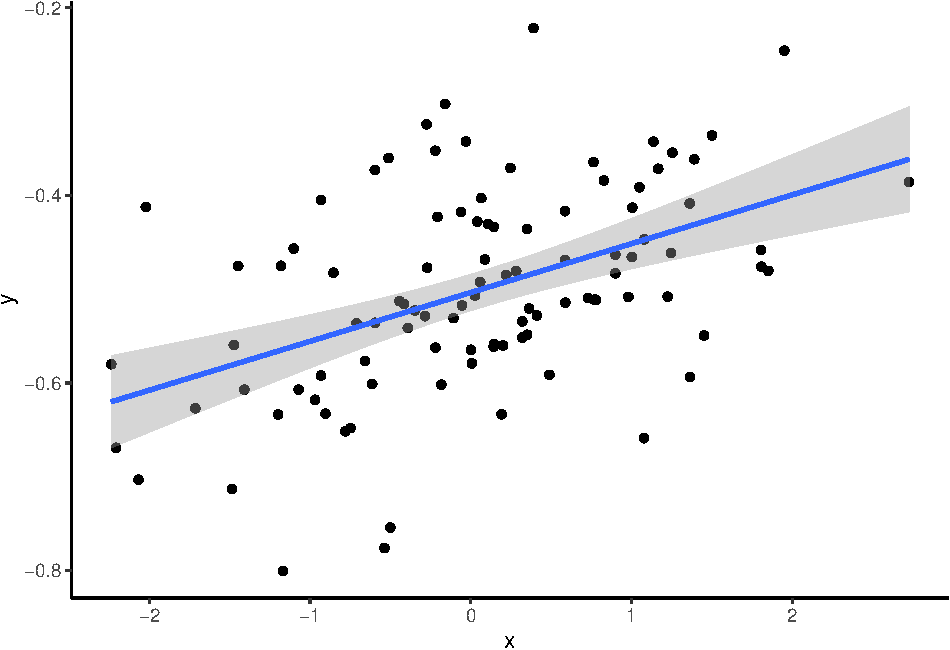
\includegraphics[width=1\linewidth]{_main_files/figure-latex/fig1-1} \caption{Figure caption}\label{fig:fig1}
\end{figure}

\pagebreak

\hypertarget{tables}{%
\section*{Tables}\label{tables}}
\addcontentsline{toc}{section}{Tables}

\begingroup\fontsize{10}{12}\selectfont

\begin{longtable}[t]{lccccccccccc}
\caption{\label{tab:tab1}My table caption}\\
\toprule
\multicolumn{1}{c}{\em{\textbf{ }}} & \multicolumn{11}{c}{\em{\textbf{High level group}}} \\
\cmidrule(l{3pt}r{3pt}){2-12}
\multicolumn{1}{c}{ } & \multicolumn{5}{c}{Group 1} & \multicolumn{6}{c}{Group 2} \\
\cmidrule(l{3pt}r{3pt}){2-6} \cmidrule(l{3pt}r{3pt}){7-12}
  & mpg & cyl & disp & hp & drat & wt & qsec & vs & am & gear & carb\\
\midrule
\endfirsthead
\caption[]{\label{tab:tab1}My table caption \textit{(continued)}}\\
\toprule
\multicolumn{1}{c}{\em{\textbf{ }}} & \multicolumn{11}{c}{\em{\textbf{High level group}}} \\
\cmidrule(l{3pt}r{3pt}){2-12}
\multicolumn{1}{c}{ } & \multicolumn{5}{c}{Group 1} & \multicolumn{6}{c}{Group 2} \\
\cmidrule(l{3pt}r{3pt}){2-6} \cmidrule(l{3pt}r{3pt}){7-12}
  & mpg & cyl & disp & hp & drat & wt & qsec & vs & am & gear & carb\\
\midrule
\endhead

\endfoot
\bottomrule
\endlastfoot
\cellcolor{gray!6}{Mazda RX4} & \cellcolor{gray!6}{21} & \cellcolor{gray!6}{6} & \cellcolor{gray!6}{160} & \cellcolor{gray!6}{110} & \cellcolor{gray!6}{3.9} & \cellcolor{gray!6}{2.6} & \cellcolor{gray!6}{16} & \cellcolor{gray!6}{0} & \cellcolor{gray!6}{1} & \cellcolor{gray!6}{4} & \cellcolor{gray!6}{4}\\
Mazda RX4 Wag & 21 & 6 & 160 & 110 & 3.9 & 2.9 & 17 & 0 & 1 & 4 & 4\\
\cellcolor{gray!6}{Datsun 710} & \cellcolor{gray!6}{23} & \cellcolor{gray!6}{4} & \cellcolor{gray!6}{108} & \cellcolor{gray!6}{93} & \cellcolor{gray!6}{3.8} & \cellcolor{gray!6}{2.3} & \cellcolor{gray!6}{19} & \cellcolor{gray!6}{1} & \cellcolor{gray!6}{1} & \cellcolor{gray!6}{4} & \cellcolor{gray!6}{1}\\
Hornet 4 Drive & 21 & 6 & 258 & 110 & 3.1 & 3.2 & 19 & 1 & 0 & 3 & 1\\
\cellcolor{gray!6}{Hornet Sportabout} & \cellcolor{gray!6}{19} & \cellcolor{gray!6}{8} & \cellcolor{gray!6}{360} & \cellcolor{gray!6}{175} & \cellcolor{gray!6}{3.1} & \cellcolor{gray!6}{3.4} & \cellcolor{gray!6}{17} & \cellcolor{gray!6}{0} & \cellcolor{gray!6}{0} & \cellcolor{gray!6}{3} & \cellcolor{gray!6}{2}\\
\addlinespace
Valiant & 18 & 6 & 225 & 105 & 2.8 & 3.5 & 20 & 1 & 0 & 3 & 1\\
\cellcolor{gray!6}{Duster 360} & \cellcolor{gray!6}{14} & \cellcolor{gray!6}{8} & \cellcolor{gray!6}{360} & \cellcolor{gray!6}{245} & \cellcolor{gray!6}{3.2} & \cellcolor{gray!6}{3.6} & \cellcolor{gray!6}{16} & \cellcolor{gray!6}{0} & \cellcolor{gray!6}{0} & \cellcolor{gray!6}{3} & \cellcolor{gray!6}{4}\\
Merc 240D & 24 & 4 & 147 & 62 & 3.7 & 3.2 & 20 & 1 & 0 & 4 & 2\\
\cellcolor{gray!6}{Merc 230} & \cellcolor{gray!6}{23} & \cellcolor{gray!6}{4} & \cellcolor{gray!6}{141} & \cellcolor{gray!6}{95} & \cellcolor{gray!6}{3.9} & \cellcolor{gray!6}{3.1} & \cellcolor{gray!6}{23} & \cellcolor{gray!6}{1} & \cellcolor{gray!6}{0} & \cellcolor{gray!6}{4} & \cellcolor{gray!6}{2}\\
Merc 280 & 19 & 6 & 168 & 123 & 3.9 & 3.4 & 18 & 1 & 0 & 4 & 4\\
\addlinespace
\cellcolor{gray!6}{Merc 280C} & \cellcolor{gray!6}{18} & \cellcolor{gray!6}{6} & \cellcolor{gray!6}{168} & \cellcolor{gray!6}{123} & \cellcolor{gray!6}{3.9} & \cellcolor{gray!6}{3.4} & \cellcolor{gray!6}{19} & \cellcolor{gray!6}{1} & \cellcolor{gray!6}{0} & \cellcolor{gray!6}{4} & \cellcolor{gray!6}{4}\\
Merc 450SE & 16 & 8 & 276 & 180 & 3.1 & 4.1 & 17 & 0 & 0 & 3 & 3\\
\cellcolor{gray!6}{Merc 450SL} & \cellcolor{gray!6}{17} & \cellcolor{gray!6}{8} & \cellcolor{gray!6}{276} & \cellcolor{gray!6}{180} & \cellcolor{gray!6}{3.1} & \cellcolor{gray!6}{3.7} & \cellcolor{gray!6}{18} & \cellcolor{gray!6}{0} & \cellcolor{gray!6}{0} & \cellcolor{gray!6}{3} & \cellcolor{gray!6}{3}\\
Merc 450SLC & 15 & 8 & 276 & 180 & 3.1 & 3.8 & 18 & 0 & 0 & 3 & 3\\
\cellcolor{gray!6}{Cadillac Fleetwood} & \cellcolor{gray!6}{10} & \cellcolor{gray!6}{8} & \cellcolor{gray!6}{472} & \cellcolor{gray!6}{205} & \cellcolor{gray!6}{2.9} & \cellcolor{gray!6}{5.2} & \cellcolor{gray!6}{18} & \cellcolor{gray!6}{0} & \cellcolor{gray!6}{0} & \cellcolor{gray!6}{3} & \cellcolor{gray!6}{4}\\
\addlinespace
Lincoln Continental & 10 & 8 & 460 & 215 & 3.0 & 5.4 & 18 & 0 & 0 & 3 & 4\\
\cellcolor{gray!6}{Chrysler Imperial} & \cellcolor{gray!6}{15} & \cellcolor{gray!6}{8} & \cellcolor{gray!6}{440} & \cellcolor{gray!6}{230} & \cellcolor{gray!6}{3.2} & \cellcolor{gray!6}{5.3} & \cellcolor{gray!6}{17} & \cellcolor{gray!6}{0} & \cellcolor{gray!6}{0} & \cellcolor{gray!6}{3} & \cellcolor{gray!6}{4}\\
Fiat 128 & 32 & 4 & 79 & 66 & 4.1 & 2.2 & 19 & 1 & 1 & 4 & 1\\
\cellcolor{gray!6}{Honda Civic} & \cellcolor{gray!6}{30} & \cellcolor{gray!6}{4} & \cellcolor{gray!6}{76} & \cellcolor{gray!6}{52} & \cellcolor{gray!6}{4.9} & \cellcolor{gray!6}{1.6} & \cellcolor{gray!6}{19} & \cellcolor{gray!6}{1} & \cellcolor{gray!6}{1} & \cellcolor{gray!6}{4} & \cellcolor{gray!6}{2}\\
Toyota Corolla & 34 & 4 & 71 & 65 & 4.2 & 1.8 & 20 & 1 & 1 & 4 & 1\\
\addlinespace
\cellcolor{gray!6}{Toyota Corona} & \cellcolor{gray!6}{22} & \cellcolor{gray!6}{4} & \cellcolor{gray!6}{120} & \cellcolor{gray!6}{97} & \cellcolor{gray!6}{3.7} & \cellcolor{gray!6}{2.5} & \cellcolor{gray!6}{20} & \cellcolor{gray!6}{1} & \cellcolor{gray!6}{0} & \cellcolor{gray!6}{3} & \cellcolor{gray!6}{1}\\
Dodge Challenger & 16 & 8 & 318 & 150 & 2.8 & 3.5 & 17 & 0 & 0 & 3 & 2\\
\cellcolor{gray!6}{AMC Javelin} & \cellcolor{gray!6}{15} & \cellcolor{gray!6}{8} & \cellcolor{gray!6}{304} & \cellcolor{gray!6}{150} & \cellcolor{gray!6}{3.1} & \cellcolor{gray!6}{3.4} & \cellcolor{gray!6}{17} & \cellcolor{gray!6}{0} & \cellcolor{gray!6}{0} & \cellcolor{gray!6}{3} & \cellcolor{gray!6}{2}\\
Camaro Z28 & 13 & 8 & 350 & 245 & 3.7 & 3.8 & 15 & 0 & 0 & 3 & 4\\
\cellcolor{gray!6}{Pontiac Firebird} & \cellcolor{gray!6}{19} & \cellcolor{gray!6}{8} & \cellcolor{gray!6}{400} & \cellcolor{gray!6}{175} & \cellcolor{gray!6}{3.1} & \cellcolor{gray!6}{3.8} & \cellcolor{gray!6}{17} & \cellcolor{gray!6}{0} & \cellcolor{gray!6}{0} & \cellcolor{gray!6}{3} & \cellcolor{gray!6}{2}\\
\addlinespace
Fiat X1-9 & 27 & 4 & 79 & 66 & 4.1 & 1.9 & 19 & 1 & 1 & 4 & 1\\
\cellcolor{gray!6}{Porsche 914-2} & \cellcolor{gray!6}{26} & \cellcolor{gray!6}{4} & \cellcolor{gray!6}{120} & \cellcolor{gray!6}{91} & \cellcolor{gray!6}{4.4} & \cellcolor{gray!6}{2.1} & \cellcolor{gray!6}{17} & \cellcolor{gray!6}{0} & \cellcolor{gray!6}{1} & \cellcolor{gray!6}{5} & \cellcolor{gray!6}{2}\\
Lotus Europa & 30 & 4 & 95 & 113 & 3.8 & 1.5 & 17 & 1 & 1 & 5 & 2\\
\cellcolor{gray!6}{Ford Pantera L} & \cellcolor{gray!6}{16} & \cellcolor{gray!6}{8} & \cellcolor{gray!6}{351} & \cellcolor{gray!6}{264} & \cellcolor{gray!6}{4.2} & \cellcolor{gray!6}{3.2} & \cellcolor{gray!6}{14} & \cellcolor{gray!6}{0} & \cellcolor{gray!6}{1} & \cellcolor{gray!6}{5} & \cellcolor{gray!6}{4}\\
Ferrari Dino & 20 & 6 & 145 & 175 & 3.6 & 2.8 & 16 & 0 & 1 & 5 & 6\\*
\end{longtable}
\endgroup{}

\pagebreak

\hypertarget{supplementaty-materials}{%
\section*{Supplementaty materials}\label{supplementaty-materials}}
\addcontentsline{toc}{section}{Supplementaty materials}

\renewcommand{\thefigure}{S\arabic{figure}}
\setcounter{figure}{0}
\renewcommand{\thetable}{S\arabic{table}}
\setcounter{table}{0}
\renewcommand{\theequation}{S\arabic{equation}}
\setcounter{equation}{0}

Lorem ipsum dolor sit amet, consectetur adipisci elit, sed eiusmod tempor incidunt ut labore et dolore magna aliqua. Ut enim ad minim veniam, quis nostrum exercitationem ullam corporis suscipit laboriosam, nisi ut aliquid ex ea commodi consequatur. Quis aute iure reprehenderit in voluptate velit esse cillum dolore eu fugiat nulla pariatur. Excepteur sint obcaecat cupiditat non proident, sunt in culpa qui officia deserunt mollit anim id est laborum.

\begin{figure}[H]
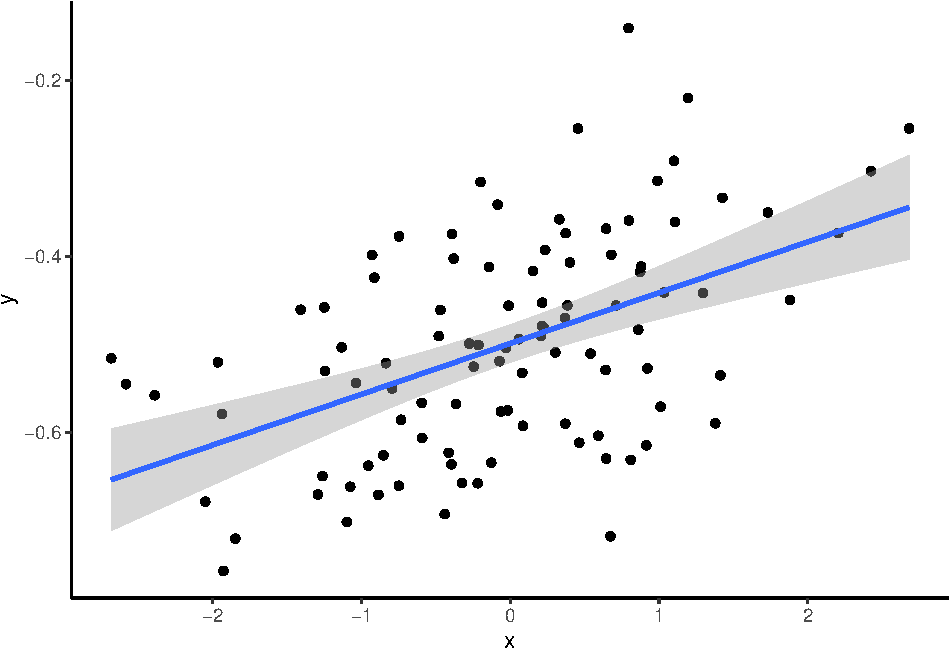
\includegraphics[width=1\linewidth]{_main_files/figure-latex/figS1-1} \caption{Figure caption}\label{fig:figS1}
\end{figure}

\end{document}
